\section{Zkoušky 2016 a 2017}
\subsection{2016}
\begin{enumerate}
    \item \textbf{Jaký musí být minimální kmitočtový zdvih $\Delta f$ modulace MSK, jestliže hodláme přenáset binární data rychlostí 100kbps}
    \begin{gather*}
        R=100 kbps \\
        \Delta f=\frac{R}{4}=25kHz
    \end{gather*}
    \item \textbf{Jaká bude šířka pásma B amplitudové modulovaného signálu SSB,  jestliže $f_d=10Hz$ a $f_h=15kHz$ a kmitočet nosné $f_c=100kHz$}

    \begin{gather*}
        \textrm{Pro SSB platí:} B = \Omega_{max} \\
        B=15kHz
    \end{gather*}
    
    \item \textbf{Určete pravděpodobnost chybného přijetí bitu P amplitudově klíčovnaého signálu ASK, je-li poměr amplitudy nosné a efektivní hodnoty šumu na vstupu součinového demodulátoru $\frac{Sc}{\sigma}=2.9$. Pravděpodobnost výskytu jedničky a nuly jsou stejné.}
    \textit{Nápověda:}
    \textit{$F_0(-3.33)=4.3423*10^{-4}$}
    \textit{$F_0(-1.67)=4.746*10^{-2}$}
    \textit{$F_0(-1.45)=7.3529*10^{-2}$}
    \textit{$F_0(-2.9)=1.8653*10^{-3}$}

    \begin{gather*}
        \textrm{Chybovost u ASK:} P_e=F_0(\frac{S_c}{2\sigma}) \\
        P_e=F_0(-1.45)=7.3529*10^{-2}
    \end{gather*}

    \item \textbf{Nakreslete blokové schéma přizpůsobeného filtru pro obdélníkový signál.} \textit{Pozn. : Ozačte šipkami směr šíření signálu}
    \begin{figure}[h!]
        \centering
        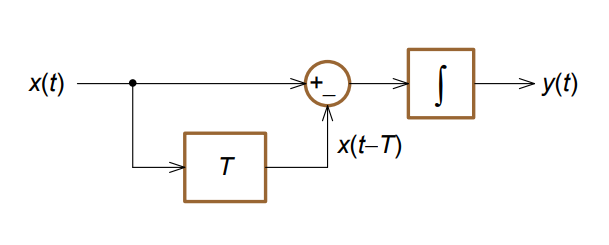
\includegraphics[scale=0.5]{images/prizfiltr.png}
        \caption{Přizpůsobený filtr}
        \label{fig:enter-label}
    \end{figure}
    \clearpage
    \item \textbf{Bipolárním signálem RZ o napětových úrovních 5 a -5 V je přenášena periodická datová posloupnost 110110110, doba trvání impulzu je poloviční oproti době trvání bitu, která je 250 $\mu s$. Určete stejnosměrnou složku a přenosovou rychlost} 
    \begin{gather*}
        T_b=250 \mu s \\
        \theta = T_b/2 \\
        A_0=5\frac{2\theta-\theta}{6\theta} \\
        A_0=\frac{5}{6} \\
        R=\frac{1}{T_b} = \frac{1}{250*10^{-6}} = 4kbps
    \end{gather*}
    \item \textbf{Jakou metodu mnohonásobného přístupu používá vysílač na následujícím obrázku? Co udává poměr přenosových rychlost $R_{ch} \textrm{ a } R_b$}
    \begin{figure}[h!]
        \centering
        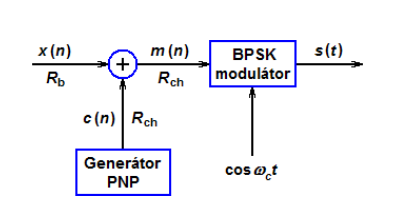
\includegraphics{images/DS.png}
        \label{fig:enter-label}
    \end{figure}
    
    - kódovou metodu
    
    - $\frac{R_ch}{R_b}$ = činitel rozprostření
    \item \textbf{Jaké rozdělení hustoty pravděpodobnosti mají okamžité hodnoty počáteční fáze úzkopásmového šumu}

    Rovnoměrné od 0 do $2\pi$ rad

    \item \textbf{Je dána amplitudová modulace DSB. Klidová amplituda nosné je 6V, hloubka je 30\%. Kmitočet modulačního signálu je 1 Hz. Modulovaný signál působí na zátěž 50 $\Omega$. Vypočtetě špičkovou hodnotu napětí modulovaného signálu. }
    \begin{gather*}
        m=\frac{\Delta S}{S_c} \\
        \Delta S =m*S_c \\
        S_{max}=S_c+\Delta S=S_c+m*S_c=6+0.3*6=7.8 
    \end{gather*}

    \item \textbf{Jakou výhodu má použití vztažného klíčování DPSK oproti BPSK.}\\
    Při nezáměrné změně fáze se chyba u DPSK projeví pouze v jednom bitu, oproti BPSK, kde dojde k obrácení celé následující sekvence.
    \item \textbf{Do připraveného grafu zakreslete modulovou kmitočtovou charekteristiku ideálního Nyquistova filtru symbolových přeslechů. Jaká hodnota činitele $\alpha$ odpovídí tomuto ideálnímu filtru?}
    \begin{figure}[h!]
        \centering
        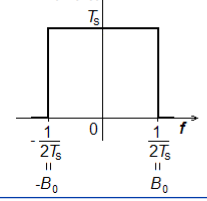
\includegraphics{images/NyqIdeal.png}
        \caption{Ideální Nyquistuv filtr}
        \label{fig:enter-label}
    \end{figure}\\
    Odpovídá $\alpha=0$
\end{enumerate}
\subsection{2017}
\begin{enumerate}
    \item \textbf{Jaká je modulační rychlost systému 32QAM, jestliže na vstup modulátoru přinášíme NRZ modulační signál s dobou trvání signálového prvku 50 $\mu s$}?
    \begin{gather*}
        N = log_2Q = log_232 = 5\\
        T_s = N \cdot \vartheta = 250\mu s\\
        M=\frac{1}{T_s}=\frac{1}{250*10^{-6}}=4 kBd  
    \end{gather*}

    \item \textbf{Nakreslete blokové schéma přizpůsobeného filtru pro pravoúhlý impulz a do připraveného grafu nakreslete jeho odezvu.}
    \begin{figure}[h!]
        \centering
        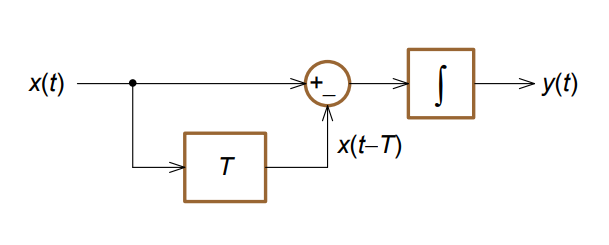
\includegraphics[scale=0.5]{images/prizfiltr.png}
        \caption{Přizpůsobený filtr}
        \label{fig:enter-label}
    \end{figure}
        \begin{figure}[h!]
        \centering
        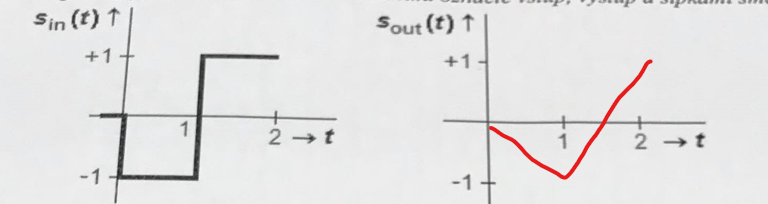
\includegraphics[scale=0.5]{images/odezva.png}
        \caption{Odezva filtru}
        \label{fig:enter-label}
    \end{figure}

    \item \textbf{Kapacita binárního kanálu je $C=0.625 SH/znak$. Stanovte nejnižší možný horní kmitočet kanálu potřebný pro přenos v základním pásmu, jestliže kapacita kanálu C' má být 1000Sh/s}
    \begin{gather*}
        C'=2f_h*C \\
        f_h=\frac{C'}{2C}=\frac{1000}{2*0.625}=800 Hz
    \end{gather*}
    \item \textbf{Nakreslete blokové schéma GMSK. Jaký musí být kmitočtový zdvih modulace, pokud má přenášet data rychlostí 64kbps.}
    \begin{gather*}
        \Delta f= \frac{R}{4}=16 kHz
    \end{gather*}
    \begin{figure}[h!]
        \centering
        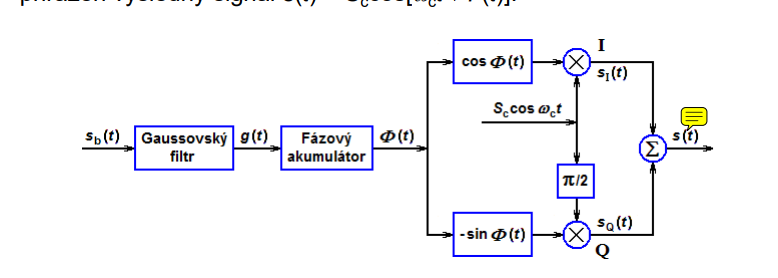
\includegraphics[scale=0.7]{images/GMSK.png}
        \caption{GMSK}
        \label{fig:enter-label}
    \end{figure}

    \item \textbf{Uvažujte osmibitovou PCM, max kmitočet je 3.4 kHz, frekvece vzorkování je 48 kHz. Rozsah signálu je od 5 do -5. Kolik bitů musí mít DPCM, aby výsledné zkreslení bylo přinejmenším stejné jako v případě PCM}
    \begin{gather*}
        \Delta_{PCM}=\Delta_{DPCM}\\
        \frac{FS}{2^N}=\frac{2\Delta_{max}}{2^N}\\
        0.039=\frac{2\Delta_{max}}{2^N}\\
        \Delta_{max}=2*D*sin(2\pi*F_{max}*T_s)=10sin(2\pi*3.4*10^3*\frac{1}{48*10^3})\\
        0.039=\frac{2*4.305}{2^N}\\
        N=log_2(\frac{2*4.305}{0.039})=7.7=8 \textrm{bitu}
    \end{gather*}

    \item \textbf{U které impulzové modulace se vykytuje jev zvaný aperturové zkreslení? 2 způsoby jak ho snížit.}
    
    PAM-F
    
    Snižujeme snížením Ts = více vzorků, předzpracováním signálu, nebo diskrétní interpolací vzorků

    \item \textbf{V osách I Q nakreslete diagram přechodů stavů $\frac{\pi}{4}$-DQPSK. Jaká může být u této modulace max změna fáze na rozhraní dvou signálových prvků}
    \begin{figure}[h!]
        \centering
        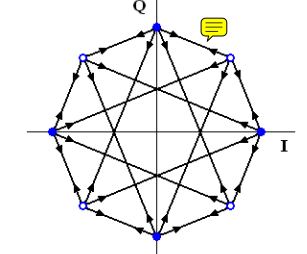
\includegraphics{images/DQPSK.png}
        \caption{DQPSK přechody}
        \label{fig:enter-label}
    \end{figure}
    
    Max přechod je 135 stupňů

    \item \textbf{Vypočtěte amplitudu první harm. složky Uni RZ signálu při přenoso posloupnosti 1111. 1 je vyjádřena kladním impulzem o výšce 5V a šířce 250 $\mu$ s následována stejně velkou mezerou. Jakou minimální šířku pásma kanálu potřebujeme pro přenos tohoto signálu}
    \begin{gather*}
        C_1=2*A_0sinc(\frac{\theta}{2}*\frac{2\pi}{T})\\
        A_0=5*\frac{\theta}{2\theta}=\frac{5}{2}\\
        C_1=5*sinc(\frac{\theta}{2}*\frac{2\pi}{2\theta})\\
        C_1=5*sinc(\frac{\pi}{2})= 3.18 \\
        B_{min}=\frac{M}{2}\\
        M=\frac{1}{T_s}\\
        B_{min}=\frac{1}{2T_s}=\frac{1}{500*10^{-6}}=2kHz
    \end{gather*}
    \item \textbf{Jmenujte alespoň dvě metody interleavingu. Jaký negativní jev způsobuje interleaving.}

    Konvoluční, blokový interleaving

    Způsobuje dopravní zpoždení

    \item \textbf{Do připraveného grafu zakreslete modulovou kmitočtovou charakteristiku raised-cosine filtru s činitel $\alpha=1$}
    \begin{figure}[h!]
        \centering
        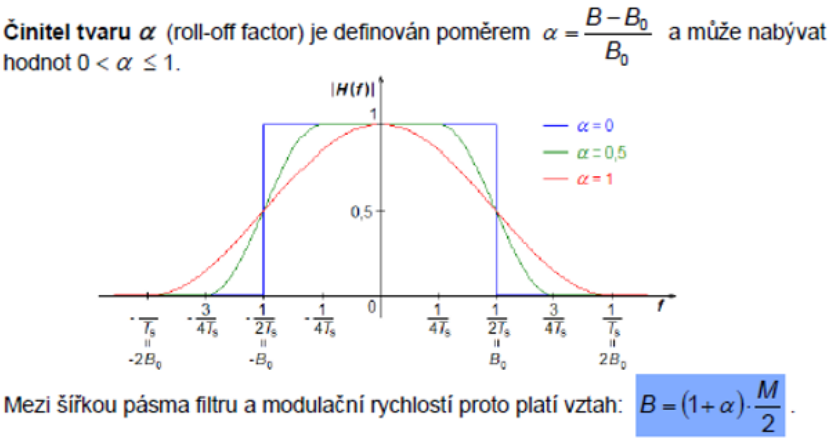
\includegraphics[scale=0.3]{images/NyquistFilter.png}
        \caption{Raised cosine filtry}
        \label{fig:enter-label}
    \end{figure}
\end{enumerate}

\subsection{Texťák z fektušky}
\begin{enumerate}
    \item \textbf{Modulace 128 QAM, kolik stavů je v kanálech I a Q}
    \begin{gather*}
        L_{I,Q}=\sqrt{Q}=\sqrt{128}=11.3= 12\textrm{ Stavů}
    \end{gather*}

    \item \textbf{Matematický vztah pro $\beta$, jakých může nabývat hodnot?????????????? }
    \begin{gather*}
        \beta=\frac{\Delta f}{F_{Max}}
    \end{gather*}
    \item \textbf{Pravděpodobnost přijetí chyby v základním pásmu}
    \begin{gather*}
        P_e=F_0(\frac{D_0-D_1}{2\sigma})
    \end{gather*}
    \item \textbf{$F_0=233kHz$ $F_1=253 kHz$, jaká je maximální šířka původního signálu.}
    \begin{gather*}
        B_{max}=\frac{f_1-f_0}{2}
    \end{gather*}
    
    \item \textbf{QAM modulace, zadán počet stavů, $T_s$, vypočítat rychlost}
    \begin{gather*}
        M=\frac{1}{T_s} \\
        R=M*log_2(Q) 
    \end{gather*}
    \item \textbf{SNR u 12 bitového převodníku, zadaná amplituda}
    \begin{gather*}
        SNR=(\frac{P_s}{P_{sum}})\\
        P_{sum}=\frac{\Delta}{12}\\
        \Delta=\frac{FS}{2^N-1}\\
        P_s=\frac{A^2}{2}
    \end{gather*}
    \item \textbf{Schéma součinového demodulátoru}
    \begin{figure}[h!]
        \centering
        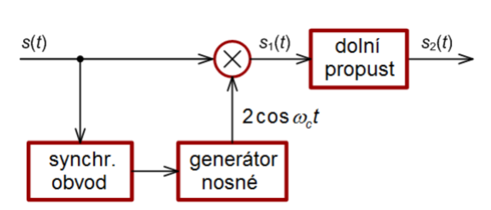
\includegraphics[width=0.5\linewidth]{images/soucindemod.png}
        \caption{Součinový demodulátor}
        \label{fig:enter-label}
    \end{figure}

    \item \textbf{Režimy ekvalizátoru}\\
      Trénink, sledování
    \item \textbf{HDB3- zakodovat sekvenci}

    Bi-rz kod, podobný  AMI, střídají se amplitudy impulzu u jedniček. V případě že je po sobě víc než tři 0, vznikne V impulz ve stejné amplitudě jako minulý impulz. Pokud by stejnosměrná složka byla nenulová, vznikne také proti impulz u další nuly do opačné amplitudy

    \item  \textbf{O jakou se jedná modulaci}\\
    \begin{figure}[h!]
        \centering
        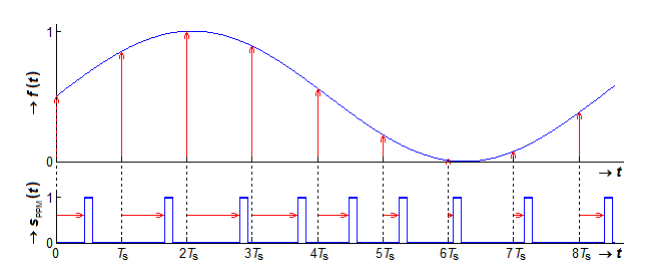
\includegraphics{images/PPM.png}
        \label{fig:enter-label}
    \end{figure}
    PPM - pulzně polohová modulace
\end{enumerate}